\begin{figure*}[!t]
  \centering

  % ---------------- Legend ----------------
  
\begin{tikzpicture}
    \begin{axis}[
      hide axis,
      xmin=0, xmax=1,
      ymin=0, ymax=1,
      legend style={
        at={(0.5,1.05)},
        anchor=south,
        legend columns=5,
        draw=none,
        font=\small
      },
    ]
      \addlegendimage{color=cyan!70, mark=square, semithick}
      \addlegendentry{HC}

      \addlegendimage{color=magenta!70, mark=square, semithick}
      \addlegendentry{HH}

      \addlegendimage{color=red!70, mark=square, semithick}
      \addlegendentry{PI}

      \addlegendimage{color=brown!70, mark=square, semithick}
      \addlegendentry{TH}

      \addlegendimage{color=blue!70, mark=square, semithick}
      \addlegendentry{QUH}
    \end{axis}
  \end{tikzpicture}

  \vspace{-1mm}

  % ---------------- Subfigure A ----------------
  \begin{subfigure}[b]{0.48\textwidth}
    \centering
    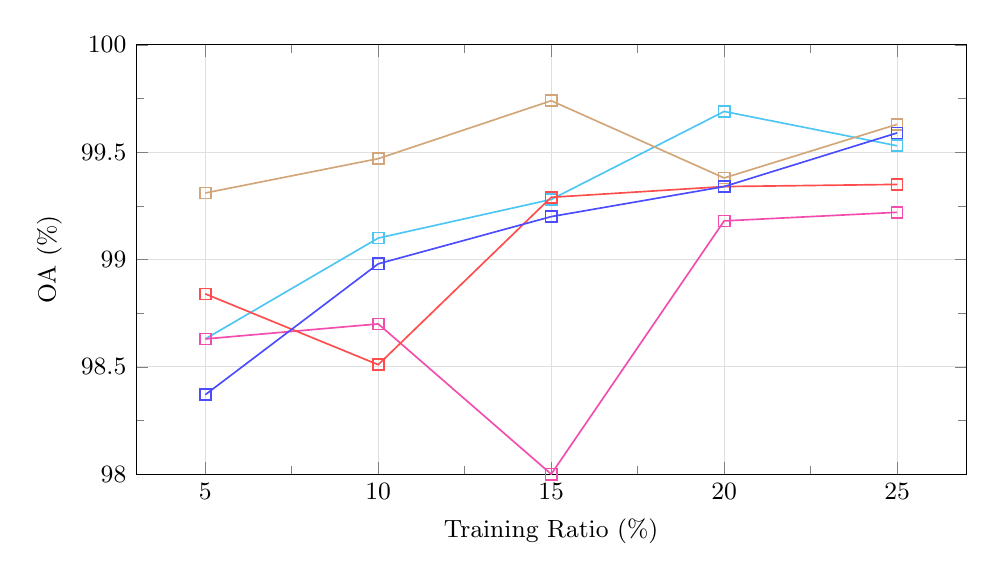
\begin{tikzpicture}
      \begin{axis}[
        width=\linewidth,
        height=0.58\linewidth,
        ylabel={OA (\%)},
        xlabel={Training Ratio (\%)},
        grid=major,
        xtick={5,10,15,20,25},
        ymin=98.0,
        ymax=100.0,
        ytick={98.0,98.5,99.0,99.5,100.0},
        minor tick num=1,
        major grid style={gray!25},
        minor grid style={gray!12},
        enlarge x limits=0.1,
        xlabel style={font=\small},
        ylabel style={font=\small},
        tick label style={font=\small},
      ]
        \addplot[color=cyan!70, mark=square, semithick] coordinates {
          (5,98.63) (10,99.10) (15,99.28) (20,99.69) (25,99.53)
        };

        \addplot[color=magenta!70, mark=square, semithick] coordinates {
          (5,98.63) (10,98.70) (15,98.00) (20,99.18) (25,99.22)
        };

        \addplot[color=red!70, mark=square, semithick] coordinates {
          (5,98.84) (10,98.51) (15,99.29) (20,99.34) (25,99.35)
        };

        \addplot[color=brown!70, mark=square, semithick] coordinates {
          (5,99.31) (10,99.47) (15,99.74) (20,99.38) (25,99.63)
        };

        \addplot[color=blue!70, mark=square, semithick] coordinates {
          (5,98.37) (10,98.98) (15,99.20) (20,99.34) (25,99.59)
        };
      \end{axis}
    \end{tikzpicture}
    \caption{Historical single-run within-scene results. OA vs. training ratio.}
    \label{fig:diff_ratio_oa}
  \end{subfigure}
  \hfill
  % ---------------- Subfigure B ----------------
  \begin{subfigure}[b]{0.48\textwidth}
    \centering
    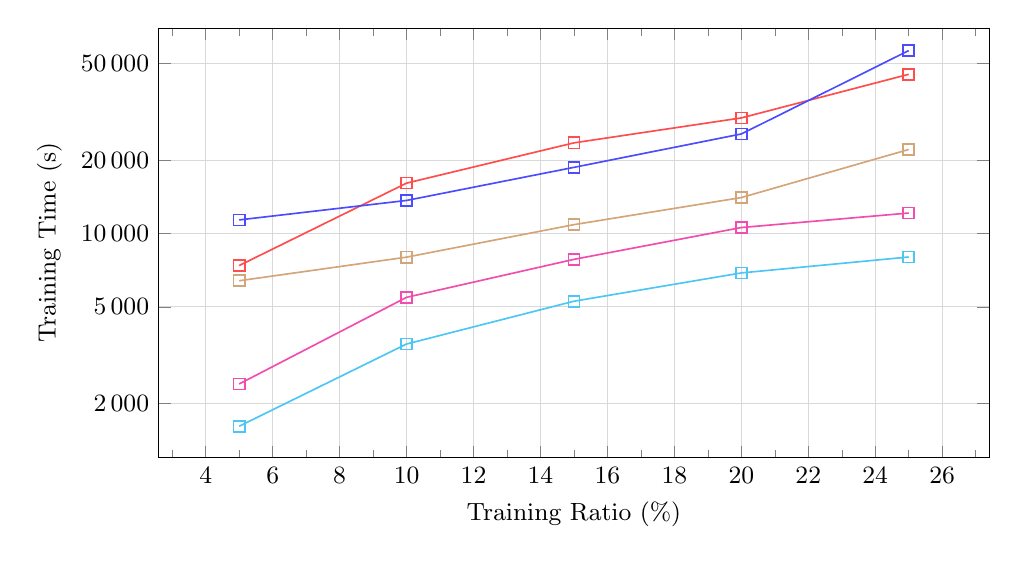
\begin{tikzpicture}
      \begin{axis}[
        width=\linewidth,
        height=0.58\linewidth,
        ylabel={Training Time (s)},
        xlabel={Training Ratio (\%)},
        ymode=log,
        ymin=1200,
        ymax=70000,
        ytick={2000,5000,10000,20000,50000},
        yticklabels={2\,000,5\,000,10\,000,20\,000,50\,000},
        scaled y ticks=false,
        grid=major,
        major grid style={gray!30},
        minor tick num=1,
        enlarge x limits=0.12,
        xlabel style={font=\small},
        ylabel style={font=\small},
        tick label style={font=\small},
      ]
        \addplot[color=cyan!70, mark=square, semithick] coordinates {
          (5,1613) (10,3515) (15,5271) (20,6892) (25,8013)
        };

        \addplot[color=magenta!70, mark=square, semithick] coordinates {
          (5,2407) (10,5469) (15,7838) (20,10593) (25,12154)
        };

        \addplot[color=red!70, mark=square, semithick] coordinates {
          (5,7391) (10,16135) (15,23627) (20,29925) (25,45229)
        };

        \addplot[color=brown!70, mark=square, semithick] coordinates {
          (5,6400) (10,8002) (15,10888) (20,14073) (25,22187)
        };

        \addplot[color=blue!70, mark=square, semithick] coordinates {
          (5,11386) (10,13691) (15,18734) (20,25701) (25,56625)
        };
      \end{axis}
    \end{tikzpicture}
    \caption{Training time vs. training ratio.}
    \label{fig:diff_ratio_time}
  \end{subfigure}

  \caption{Training ratio--accuracy--efficiency trade-off of FKANMamba on five HSI benchmarks.}
  \label{fig:diff_ratio}
\end{figure*}


















% \begin{figure*}[!htbp]
%   \centering
%   % Common legend 
%   \begin{tikzpicture}
%     \begin{axis}[
%       hide axis,
%       xmin=0, xmax=1, ymin=0, ymax=1,
%       legend style={at={(0.5,1.1)}, anchor=south, legend columns=-1},
%     ]
%       \addlegendimage{cyan!70, mark=square, semithick} \addlegendentry{HC}
%       \addlegendimage{magenta!70, mark=square, semithick} \addlegendentry{HH}
%       \addlegendimage{red!70, mark=square, semithick} \addlegendentry{PI}
%       \addlegendimage{brown!70, mark=square, semithick} \addlegendentry{TH}
%       \addlegendimage{blue!70, mark=square, semithick} \addlegendentry{QUH}
%     \end{axis}
%   \end{tikzpicture}

%   \begin{subfigure}[b]{0.48\textwidth}
%     \centering
%     % Added trim axis left/right to normalize the plot area
%     \begin{tikzpicture}[trim axis left, trim axis right]
%       \begin{axis}[
%         width=\textwidth,
%         height=0.55\textwidth,
%         ylabel={OA (\%)},
%         xlabel={Training Ratio (\%)},
%         grid=major,
%         xtick={5,10,15,20,25},
%         ymin=98.0, ymax=100.0,
%         ytick={98.0,98.5,99.0,99.5,100.0},
%         minor tick num=1,
%         major grid style={gray!25},
%         minor grid style={gray!12},
%         enlarge x limits=0.1,
%         xlabel style={font=\small},
%         ylabel style={font=\small},
%         tick label style={font=\small},
%       ]
%         \addplot[color=cyan!70, mark=square, semithick] coordinates {(5,98.63) (10,99.10) (15,99.28) (20,99.69) (25,99.53)} ;
%         \addplot[color=magenta!70, mark=square, semithick] coordinates {(5,98.63) (10,98.70) (15,98.00) (20,99.18) (25,99.22)};
%         \addplot[color=red!70, mark=square, semithick] coordinates {(5,98.84) (10,98.51) (15,99.29) (20,99.34) (25,99.35)};
%         \addplot[color=brown!70, mark=square, semithick] coordinates {(5,99.31) (10,99.47) (15,99.74) (20,99.38) (25,99.63)};
%         \addplot[color=blue!70, mark=square, semithick] coordinates {(5,98.37) (10,98.98) (15,99.20) (20,99.34) (25,99.59)};
%       \end{axis}
%     \end{tikzpicture}
%   \end{subfigure}
%   \hfill
%   \begin{subfigure}[b]{0.48\textwidth}
%     \centering
%     \begin{tikzpicture}[trim axis left, trim axis right]
%       \begin{axis}[
%         width=\textwidth,
%         height=0.55\textwidth,
%         ylabel={Training Time (s)},
%         xlabel={Training Ratio (\%)},
%         ymode=log,
%         ymin=1200, ymax=70000,
%         ytick={2000,5000,10000,20000,50000},
%         yticklabels={2\,000,5\,000,10\,000,20\,000,50\,000},
%         scaled y ticks=false,
%         grid=major,
%         major grid style={gray!30},
%         minor tick num=1,
%         enlarge x limits=0.12,
%         xlabel style={font=\small},
%         ylabel style={font=\small},
%         tick label style={font=\small},
%       ]
%         \addplot[color=cyan!70, mark=square, semithick] coordinates {(5,1613) (10,3515) (15,5271) (20,6892) (25,8013)};
%         \addplot[color=magenta!70, mark=square, semithick] coordinates {(5,2407) (10,5469) (15,7838) (20,10593) (25,12154)};
%         \addplot[color=red!70, mark=square, semithick] coordinates {(5,7391) (10,16135) (15,23627) (20,29925) (25,45229)};
%         \addplot[color=brown!70, mark=square, semithick] coordinates {(5,6400) (10,8002) (15,10888) (20,14073) (25,22187)};
%         \addplot[color=blue!70, mark=square, semithick] coordinates {(5,11386) (10,13691) (15,18734) (20,25701) (25,56625)};
%       \end{axis}
%     \end{tikzpicture}
%   \end{subfigure}
%   \caption{Training ratio–accuracy–efficiency trade-off of FKANMamba on five HSI benchmarks.}
%   \label{diff_ratio}
% \end{figure*}










% THe previous Nature sTtyle
% \begin{figure}[ht]
%   \centering
%   \begin{tikzpicture}
%     % Common legend style
%     \begin{axis}[
%       hide axis, % invisible dummy axis just for legend
%       xmin=0, xmax=1, ymin=0, ymax=1,
%       legend style={at={(0.5,1.1)}, anchor=south, legend columns=-1},
%     ]
%       \addlegendimage{cyan!70, mark=square, semithick} \addlegendentry{HC}
%       \addlegendimage{magenta!70, mark=square, semithick} \addlegendentry{HH}
%       \addlegendimage{red!70, mark=square, semithick} \addlegendentry{PI}
%       \addlegendimage{brown!70, mark=square, semithick} \addlegendentry{TH}
%       \addlegendimage{blue!70, mark=square, semithick} \addlegendentry{QUH}
%     \end{axis}
%   \end{tikzpicture}

%   \begin{subfigure}[b]{0.48\textwidth}
%     \centering
%     \begin{tikzpicture}
%       \begin{axis}[
%         width=\textwidth,
%         height=0.55\textwidth,
%         ylabel={OA (\%)},
%         xlabel={Training Ratio (\%)},
%         grid=major,
%         xtick={5,10,15,20,25},
%         ymin=98.0, ymax=100.0,
%         ytick={98.0,98.5,99.0,99.5,100.0},
%         minor tick num=1,
%         major grid style={gray!25},
%         minor grid style={gray!12},
%         enlarge x limits=0.1,
%         xlabel style={font=\small},
%         ylabel style={font=\small},
%         tick label style={font=\small},
%       ]
%         \addplot[color=cyan!70, mark=square, semithick] coordinates {
%           (5,98.63) (10,99.10) (15,99.28) (20,99.69) (25,99.53) } ; %HC
%         \addplot[color=magenta!70, mark=square, semithick] coordinates {
%           (5,98.63) (10,98.70) (15,98.00) (20,99.18) (25,99.22)  }; %HH
%         \addplot[color=red!70, mark=square, semithick] coordinates {
%           (5,98.84) (10,98.51) (15,99.29) (20,99.34) (25,99.35) }; %PI
%         \addplot[color=brown!70, mark=square, semithick] coordinates {
%           (5,99.31) (10,99.47) (15,99.74) (20,99.38) (25,99.63)}; %TH
%         \addplot[color=blue!70, mark=square, semithick] coordinates {
%           (5,98.37) (10,98.98) (15,99.20) (20,99.34) (25,99.59)}; % QUH
%       \end{axis}
%     \end{tikzpicture}
%     % \caption{OA vs Training ratio}
%     \label{Fig1A}
%   \end{subfigure}
%   \hfill
%   \begin{subfigure}[b]{0.48\textwidth}
%     \centering
%     \begin{tikzpicture}[trim axis left, trim axis right]
%       \begin{axis}[
%         width=\textwidth,
%         height=0.55\textwidth,
%         ylabel={Training Time (s)},
%         xlabel={Training Ratio (\%)},
%         ymode=log,
%         ymin=1200, ymax=70000,
%         ytick={2000,5000,10000,20000,50000},
%         yticklabels={2\,000,5\,000,10\,000,20\,000,50\,000},
%         scaled y ticks=false,
%         grid=major,
%         major grid style={gray!30},
%         minor tick num=1,
%         enlarge x limits=0.12,
%         xlabel style={font=\small},
%         ylabel style={font=\small},
%         tick label style={font=\small},
%       ]
%         \addplot[color=cyan!70, mark=square, semithick] coordinates {
%           (5,1613) (10,3515) (15,5271) (20,6892) (25,8013)};%HC
%         \addplot[color=magenta!70, mark=square, semithick] coordinates {
%          (5,2407) (10,5469) (15,7838) (20,10593) (25,12154) }; %HH
%         \addplot[color=red!70, mark=square, semithick] coordinates {
%           (5,7391) (10,16135) (15,23627) (20,29925) (25,45229)}; %PI
%         \addplot[color=brown!70, mark=square, semithick] coordinates {
%           (5,6400) (10,8002) (15,10888) (20,14073) (25,22187) }; %TH
%         \addplot[color=blue!70, mark=square, semithick] coordinates {
%           (5,11386) (10,13691) (15,18734) (20,25701) (25,56625)}; %QUH
%       \end{axis}
%     \end{tikzpicture}
%     % \caption{Training Time vs Training Ratio}
%     \label{Fig1B}
%   \end{subfigure}
%   \caption{ Training ratio–accuracy–efficiency trade-off of FKANMamba on five HSI benchmarks.}
%   \label{fig:diff_ratio}
% \end{figure}
